\section{Beispiele}

\subsection*{Übertragungsmedien}

\begin{example2}{Bandbreite von Twisted-Pair Kabeln}

Bei allen TP Kabelkategorien steigt der Dämpfungsbelag mit zunehmender Frequenz beinahe gleich an

Was ist der Grund, dass CAT5 Kabel mit einer Bandbreite von100 MHz verwendet werden, während CAT7 Kabel bis zu 600 MHz eingesetzt werden?

\emph{Antwort:}
Die Dämpfung ist nicht die einzige Grösse, welche die effektiv nutzbare Bandbreite eines Kabels bestimmt. Höherwertige Kabel habe eine viel besseres Übersprechverhalten, so dass eine höhere Dämpfung akzeptiert werden kann.
\end{example2}

\begin{example2}{Optische Übertragungsmedien}\\
  Die optische Sendeeinrichtung sendet mit $10^{-3}$ Watt Leistung. Für eine genügende Übertragungsqualität muss
  der Leistungspegel beim Empfänger mindestens $10^{-5}$ Watt betragen. Der Lichtwellenleiter hat einen
  Dämpfungsbelag von $0.5 \mathrm{~dB} / \mathrm{km}$. Welche Distanz kann überbrückt werden?

 \textbf{Antwort:}
Die erlaubte Abschwächung der Leistung entspricht dem Faktor 100, also $20 \mathrm{~dB}$. Demzufolge darf die Leitung maximal $40 \mathrm{~km}$ lang sein.
\end{example2}

\subsection*{OSI Modell}

\begin{example2}{Klassifizierung von Diensten}
  Zwei Schichten M und N haben zur jeweils höheren Schicht die folgenden Interfaces. Klassifizierung der Dienste?

  \vspace{1mm}

  M:

connect\_M (dest\_addr, options, \&handle)\\
send\_M (handle, options, numBytes, \&data)\\
..\\
close\_M (handle)

\emph{Antwort:} verbindungsorientiert, Connect/Close der Verbindung

\vspace{1mm}

N:

send\_telegramm\_N (remote\_addr, numBytes, \&data)\\
receive\_telegram\_N (\&remote\_addr, \&local\_address, \&buffer, bufsiz)

\emph{Antwort:} verbindungslos, keine Funktion zum Auf-/Abbau einer Verb.
\end{example2}

\subsection*{Physical Layer}

\begin{example}
    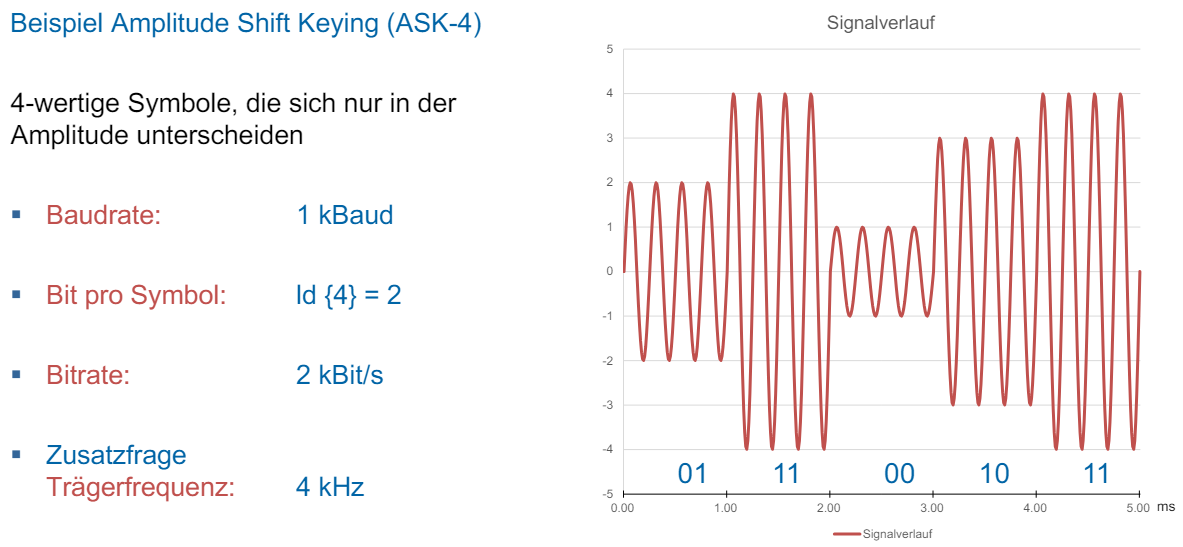
\includegraphics[width=1\linewidth]{images/images/amplitude_shift_keying.png}
\end{example}

\begin{example2}{Maximale Bitrate}
  Ein Übertragungssystem nutzt eine Bandbreite von $100 \mathrm{MHz}$ und codiert den Bitstrom mit 4wertigen Symbolen.
 
  Welches ist die theoretisch erreichbare maximale Bitrate?
 
 \textbf{Antwort:}
 $max_{Symbolrate} =200 \mathrm{MBd}$\\
 2 Bit/Symbol $\rightarrow$ $max_{Bitrate}$ $=400 \mathrm{Mbit} / \mathrm{s}$
 
 \vspace{2mm}
 
 Zur Steigerung der Bitrate wird ein 8-wertiger Code in Erwägung gezogen. Unter welchen Voraussetzungen ist das möglich?
 
 \textbf{Antwort:}
 Der Signal/Rauschabstand S/N muss genügend gross sein. Das ergibt sich aus der Sendeleistung, der Leitungsdämpfung und der Störleistung
 \end{example2}


 \begin{example2}{Maximale Zeichenrate}
 Wir betrachten eine asynchrone Schnittstelle, welche mit folgenden Parametern betrieben wird: Bitdauer T ist $1 \mathrm{~ms}$, 8 Bit/Zeichen, 1 Stopp-Bit.
 
 a) Welche maximale Zeichenrate lässt die Schnittstelle zu?
 
 \textbf{Antwort:}
 1000 Bit/s / 10 Bit/Zeichen = 100 Zeichen/s
 
 b) Um wieviel darf die Frequenz des Empfängertaktgebers von dem des Senders maximal abweichen, ohne dass das einen Übertragungsfehler bewirkt? Relative Angabe in Prozent.
 
 \textbf{Antwort:}
 Zeitmessung startet mit der fallenden Flanke des Start-Bits nach 9.5*T ist man im Idealfall in der Mitte des letzten Datenbits,
 Fehlablesung entsteht dann, wenn man um 0.5*T daneben liegt $\rightarrow 0.5 * \mathrm{~T} / 9.5 * \mathrm{~T}=1 / 19=5.26 \%$

 c) Wir betrachten den Fall, bei dem die Frequenz des Empfängertaktgebers geringfügig höher ist, als der unter b) errechnete Wert. Es wird das Zeichen 10101010 gesendet. Welches Zeichen detektiert der Empfänger?

 \textbf{Antwort:}
Das zuletzt übertragene Bit wird nicht abgetastet, dafür das vorhergehende zweimal. Weil das letzte Bit das MSB ist, wird das Zeichen 00101010 empfangen.
 \end{example2}



 \begin{example2}{Codierung auf Leitungen}

  a) Welche Eigenschaft muss ein Leitungscode aufweisen, dass der Empfänger den Takt aus dem Datenstrom extrahieren kann?
  
  \textbf{Antwort:} Der Bitstrom muss so codiert werden, dass er - unabhängig von den übertragenen Daten - genügend häufige Pegeländerungen (Signalflanken) aufweist.
  
  b) Nennen Sie zwei Codes, welche die Bedingung unter a) erfüllen.
  
  \textbf{Antwort:} Manchester (10Base2, 10BASE-T), dreiwertiger NRZI mit 4B5B Codierung (100Base-TX), 4B3T (10BASE-T1L)
  
  c) Aus welchen Gründen kann es notwendig sein, dass ein Leitungscode gleichstromfrei ist? 
  
  \textbf{Antwort:} Wird das Signal galvanisch getrennt über einen Transformator geführt wird, dann geht der Gleichstromanteil verloren.
  
  d) Nennen Sie zwei Codes, welche gleichstromfrei sind. \textbf{Antwort:} AMI, 4B3T (10BASE-T1L), dreiwertiger NRZI (100Base-T)
 \end{example2}

 \begin{example2}{Ein Übertragungsverfahren}
  soll 320 MBit/s übertragen können. Die im Übertragungsmedium nutzbare Bandbreite $B$ beträgt $40 \mathrm{MHz}$.

Wie viele Zustände pro Symbol muss das Codierungsverfahren bieten, damit bei maximaler Symbolrate die geforderte Bitrate erreicht werden kann? 

\textbf{Antwort:}
Hartley: Bitrate $=2$ * $B$ * $\operatorname{Id}(\mathrm{N})$

$\rightarrow 320 \mathrm{Mb} / \mathrm{s}<=80 \mathrm{MHz}$ * Id $(\mathrm{A})$

$\rightarrow \operatorname{Id}(A)>=4$ Damit werden mindestens $2 * * 4=16$ Zustände benötigt.
 \end{example2}

\subsection*{Data Link Layer}

\begin{example2}{Datenübertragung und Framing}\\
    Gegeben: Bitrate 100 Mbit/s, Frame-Länge 1000 Byte, IFG 96 Bit, Payload 800 Byte. Berechnen Sie die Nutzdatenrate.\\
    \textbf{Lösung:}\\
    $$F_R = \frac{100 \cdot 10^6}{8 \cdot (1000 + 96)} = 1.19 \cdot 10^6 \text{ Frames/s}$$
    $$N = 1.19 \cdot 10^6 \cdot 800 \cdot 8 = 7.6 \cdot 10^9 \text{ Bit/s} = 7.6 \text{ Gbit/s}$$
\end{example2}

 \begin{example2}{Bitstuffing}
  Synchrone Datenübertragung und Codes
  
  Bei der synchronen Datenübertragung werde das Flag 01111110 und Bit-Stuffing (Bitstopfen) verwendet.
  
  a) Wozu verwendet man hier Bit-Stuffing?
  
  \textbf{Antwort:}
  Start-/Ende-Flags dürfen nicht in den eigentlichen Daten vorkommen, da dies vom Empfänger als Flag detektiert würde
  
  b) Wie sieht der folgende gesendete Bitstrom auf der Leitung aus?
  
  \textbf{Antwort:}

  1010111111010011111111111000000101011111011111101
  
  10101111\textbf{0}1010011111\textbf{0}11111\textbf{0}11000000101011111\textbf{0}011111\textbf{0}101
  \end{example2}

  \begin{example2}
    {Fehlerkorrektur beim Stop-and-Wait Protokoll}

  Der Sender erkennt durch einen Timeout eine fehlende Bestätigung und wiederholt daraufhin das zuletzt gesendete Telegramm.
  \end{example2}

\subsection*{LAN und Ethernet}

\begin{formula}{GBASE-T}\\
    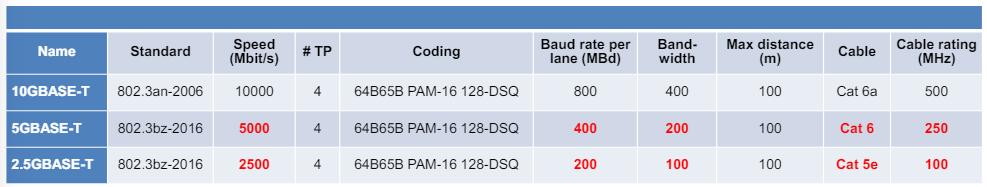
\includegraphics[width=1\linewidth]{images/images/GBASE-T.png}
\end{formula}

\begin{example2}{100Base-TX Kabel und Stecker}

  Charakterisieren Sie das für 100 Base-TX verwendete Kabel (inkl. Stecker). Worin können sich solche Kabel unterscheiden?

- UTP (Kabel, das ungeschirmte verdrillte Aderpaare enthält). Das universell verwendbare Kabel enthält 8 Adern, von denen bei 100 Base-TX nur 4 verwendet werden.

- Üblicher Stecker ist vom Typ RJ45.

- Unterschiede: Es gibt 1:1 und Crossover - Kabel. Die Übertragungseigenschaften können sehr verschieden sein und werden durch die Kabelkategorie charakterisiert.
\end{example2}

\begin{example2}{100Base-TX Oszilloskop}\\
 Sie sehen auf einem Oszilloskop das folgende Bild eines 100Base-TX Signals:
  \begin{center}
  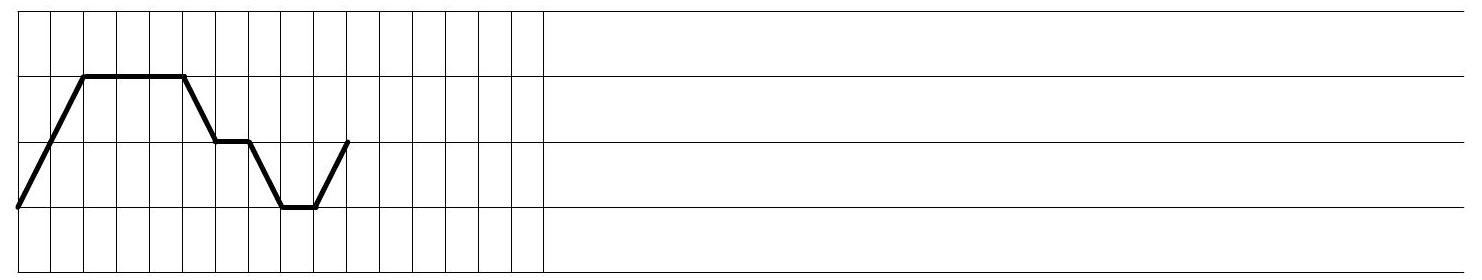
\includegraphics[width=0.8\linewidth]{images/images/2024-06-20-17-47-36.png}
  \end{center}
Ein Kästchen entspricht einem Bit. Wie lauten die ersten 10 Bits?

\textbf{Antwort:}
1100010101
\end{example2}


\begin{example2}{Ethernet Segment Rate}
Wie viele Frames pro Sekunde können auf einem 100 Base-TX Ethernet Segment pro Richtung maximal übertragen werden?
Hinweis: Denke an Inter-Frame Gap, die mindestens so lange wie die Übertragung von 12 Bytes dauert.

\textbf{Antwort:}
Die grösste Frame Rate wird erreicht, wenn alle Frames die minimale Länge von 64 Oktetts aufweisen. Solche Frames belegen folgende Anzahl von Oktett Einheiten von 80 ns:

- 8 für Präambel und Start Frame Delimiter (SFD)\\
- 64 für das eigentliche Frame (mit bis zu 46 Oktetts Nutzdaten)\\
- 12 für Interframe Gap ( 960 ns)

Framerate $=10^{8}$ bit per second $/ 8$ * $(8+64+12)$ bit per frame $=148$ ' 800 frames per second
\end{example2}


\begin{example2}{Transit Delay}
Wir betrachten ein sehr schwach belastetes Ethernet (d.h. praktisch keine Kollisionen und keine Wartezeiten in Switches). Worin besteht der wesentliche Unterschied, ob man nun ein $100 \mathrm{Mb} / \mathrm{s}$ oder ein Gigabit-Ethernet verwendet? Wo ist dieser Unterschied wichtig?

\textbf{Antwort:}
Transit Delay ist im 1000 Mb/s-Ethernet 10 mal geringer, was bei kaskadierten Store and Forward Switches erheblich sein kann. Die resultierende Round Trip Time kann die Performance stark beeinflussen. $1000 \mathrm{Mb} / \mathrm{s}$-Ethernets haben nicht nur einen höheren Durchsatz, sie sind auch reaktionsfreudiger!

Beispiel: 3 Switches und maximal langes Frame $\rightarrow 4 * 12.3 \mu \mathrm{s}$ versus $4 * 123 \mu \mathrm{s}$
\end{example2}

\begin{example2}{Filtering Database}
  Ein Netzwerk besteht aus einem Ethernet Switch, drei Ethernet Hubs und 10 Endgeräten. Anfangsbedingung: Der Ethernet Switch kennt zu Beginn keine einzige MAC-Adresse. Annahmen: Die Aging-Time betrage 300 Sekunden. Die Aging-Time für eine MAC-Adresse wird nur zurückgesetzt, wenn diese MAC-Adresse als Quelladresse erscheint.

\vspace{1mm}

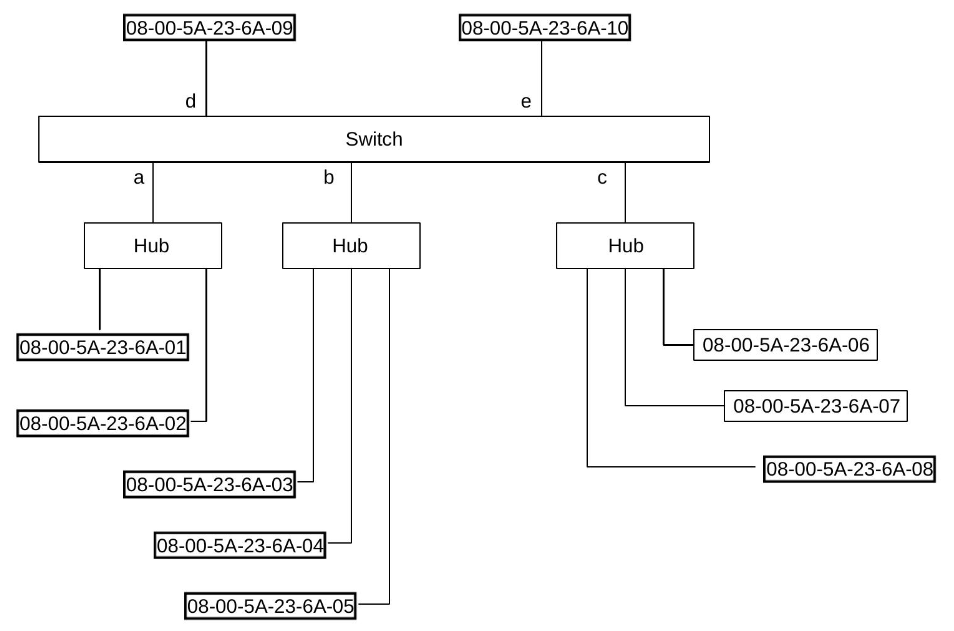
\includegraphics[width=0.9\linewidth]{images/images/bsp_filtering_database1.png}

Auf welchen Switchports (a ... e) sind die Meldungen sichtbar?

\vspace{1mm}

\resizebox{\linewidth}{!}{
  \begin{tabular}{|c|c|l|l|l|l|l|l|l|}
    \hline Zeit t & Nr. & Quelladresse & Zieladresse & a & b & c & d & e \\
    \hline 0 & 1 & $08-00-5 A-23-6 A-01$ & $08-00-5 A-23-6 A-10$ & $x$ & $x$ & $x$ & $x$ & $x$ \\
    \hline $10 \mathrm{~s}$ & 2 & $08-00-5 A-23-6 A-05$ & $08-00-5 A-23-6 A-01$ & $x$ & $x$ & & & \\
    \hline $20 \mathrm{~s}$ & 3 & $08-00-5 A-23-6 A-09$ & $08-00-5 A-23-6 A-08$ & $x$ & $x$ & $x$ & $x$ & $x$ \\
    \hline $30 \mathrm{~s}$ & 4 & $08-00-5 A-23-6 A-07$ & $08-00-5 A-23-6 A-04$ & $x$ & $x$ & $x$ & $x$ & $x$ \\
    \hline $120 \mathrm{~s}$ & 5 & $08-00-5 A-23-6 A-09$ & $08-00-5 A-23-6 A-05$ & & $x$ & & $x$ & \\
    \hline $250 \mathrm{~s}$ & 6 & $08-00-5 A-23-6 A-06$ & $08-00-5 A-23-6 A-01$ & $x$ & & $x$ & & \\
    \hline $260 \mathrm{~s}$ & 7 & $08-00-5 A-23-6 A-03$ & $08-00-5 A-23-6 A-09$ & & $x$ & & $x$ & \\
    \hline $320 \mathrm{~s}$ & 8 & $08-00-5 A-23-6 A-03$ & $08-00-5 A-23-6 A-07$ & & $x$ & $x$ & & \\
    \hline $350 \mathrm{~s}$ & 9 & $08-00-5 A-23-6 A-09$ & $08-00-5 A-23-6 A-07$ & $x$ & $x$ & $x$ & $x$ & $x$ \\
    \hline $400 \mathrm{~s}$ & 10 & $08-00-5 A-23-6 A-02$ & $08-00-5 A-23-6 A-06$ & $x$ & & $x$ & & \\
    \hline
    \end{tabular}}
\end{example2}


\begin{example2}{Interpretation eines Hex-Dumps (MAC-Frame)}
  Hex-Dump eines MAC-Frames, wie er mit Wireshark aufgezeichnet worden ist:

  \vspace{1mm}

\resizebox{\linewidth}{!}{
\begin{tabular}{lllllllllllllllll}
$0000:$ & 08 & 00 & $2 B$ & $C 3$ & $A C$ & $A 5$ & 00 & 00 & $F 8$ & $1 A$ & 84 & $1 A$ & 08 & 00 & 45 & 00 \\
$0010:$ & 00 & $2 C$ & $1 B$ & 31 & 40 & 00 & 80 & 06 & 99 & $5 E$ & $A 0$ & 55 & 82 & $2 A$ & $A 0$ & 55 \\
$0020:$ & 83 & 67 & 04 & $1 A$ & 12 & 67 & 00 & 00 & C0 & C5 & 00 & 00 & 00 & 00 & 60 & 02 \\
$0030:$ & 20 & 00 & $5 A$ & $A 3$ & 00 & 00 & 02 & 04 & 05 & $B 4$ & 00 & 00 & $A 3$ & $7 C$ & 51 & FB
\end{tabular}}

\vspace{1mm}

a) Markieren und benennen Sie die einzelnen Felder.

Oktett 0-5: Destination MAC-Address (08-00-2B-C3-AC-A5)

Oktett 6-11: Source MAC-Address (00-00-F8-1A-84-1A)

Oktett 12/13: Length / Type $\rightarrow$ hier Type $=0 \times 0800$

Oktett 14-59: Data / padding

Oktett 60-63: Frame Check Sequence

b) Was lässt sich über den Inhalt des Datenfeldes aussagen?
\textbf{Antwort:}
ein IP-Paket (wegen Type $=0 x 0800$ )
\end{example2}


\subsection*{Network Layer}

\begin{example2}{Routingtabelle}
  Gegeben ist folgendes Netzwerk:

  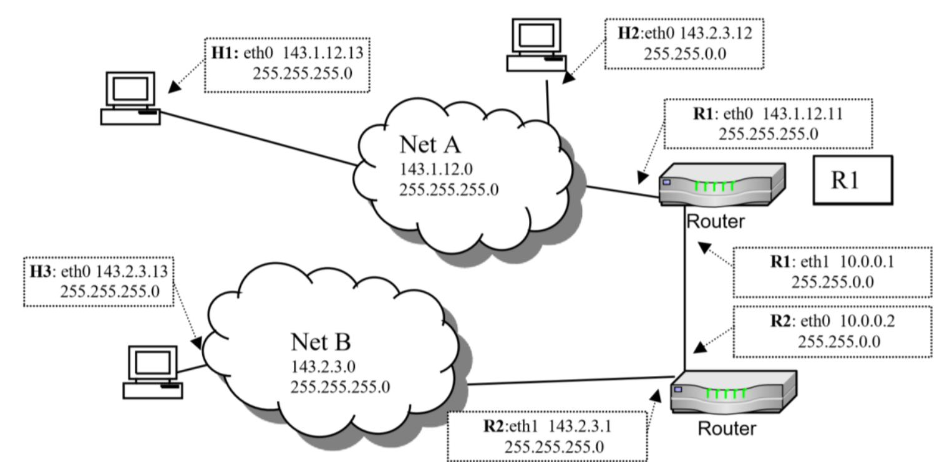
\includegraphics[width=0.8\linewidth]{images/images/bsp_routing.png}

  Routingtabelle von Host H1:

  \begin{tabular}{llll} 
    Netzadresse & Netzmaske & Interface & Gateway \\
    143.1.12.0 & 255.255 .255 .0 & eth0 & (direkt) \\
    default & & eth0 & 143.1 .12 .11
    \end{tabular}\\

    a) Host $\mathrm{H} 1$ pingt Host $\mathrm{H} 2$ mit ping 143.2.3.12, bekommt jedoch keine Antwort, obwohl alle Router richtig konfiguriert sind. Warum nicht? 

$\mathrm{H} 2$ hat falsche Subnetzmaske und hat eine Adresse vom Netz B.
Daraus folgt: H1 sendet das Paket zum Router anstatt ins angrenzende Netz.
Das Paket wird zu Router R2 weitergeleitet, der in Netz B keinen entsprechenden Host findet.

b) Routing-Tabelle von Router R1:

\begin{tabular}{llll} 
Netzadresse & Netzmaske & Interface & Gateway \\
143.1 .12 .0 & 255.255 .255 .0 & eth0 & (direkt) \\
10.0 .0 .0 & 255.255 .0 .0 & eth1 & (direkt) \\
143.2 .3 .0 & 255.255 .255 .0 & eth1 & 10.0 .0 .2
\end{tabular}\\

c) Warum kann der Host $\mathrm{H} 3$ den Host $\mathrm{H} 2$ nicht erreichen? In welchem Subnetz sucht $\mathrm{H} 3$ den Zielhost? Welchen Weg beschreitet das „Ping-Paket“(Gehen Sie davon aus, dass die Routingtabellen in allen Komponenten vollständig gemäss den Einträgen aus obigem Netzdiagramm generiert wurden).

$\mathrm{H} 3$ sucht H2 im Netz B, d.h. der Ping wird nicht über den Router gesendet. H2 erhält somit die Anfrage nicht.
\end{example2}

\begin{example2}{IP Subnetz Aufteilung}\\
Sie bekommen von Ihrem Internet Service Provider (ISP) ein privates Klasse-C Netz zugeteilt. In Ihrem Haus befinden sich 4 Parteien, welche sich den Internet-Anschluss teilen. Sie geben jeder Partei ein gleich grosses Subnetz, indem sie das Klasse-C Netz 192.168.1.0/24 in 4 Subnetze aufteilen. Geben Sie für alle 4 Subnetze die Netzadresse, die Netzmaske, die Broadcast-Adresse, den Default Gateway sowie die Anzahl adressierbarer Hosts an.


\begin{minipage}{0.5\linewidth}
  \resizebox{\linewidth}{!}{
  \begin{tabular}{|l|l|}
    \hline \multicolumn{2}{|l|}{ Subnetz 1 } \\
    \hline Netzadresse & 192.168.1.0 \\
    \hline Broadcast-Adresse & 192.168.1.63  \\
    \hline
    \end{tabular}}
    
    \resizebox{\linewidth}{!}{
    \begin{tabular}{|l|l|}
    \hline \multicolumn{2}{|l|}{ Subnetz 2} \\
    \hline Netzadresse & 192.168.1.64 \\
    \hline Broadcast-Adresse & 192.168.1.127 \\
    \hline
    \end{tabular}}  
\end{minipage}
\begin{minipage}{0.5\linewidth}
  \resizebox{\linewidth}{!}{
    \begin{tabular}{|l|l|}
      \hline \multicolumn{2}{|l|}{ Subnetz 3 } \\
      \hline Netzadresse & 192.169.1.128 \\
      \hline Broadcast-Adresse & 192.168.1.191 \\
      \hline
      \end{tabular}}
      
      \resizebox{\linewidth}{!}{
      \begin{tabular}{|l|l|}
      \hline \multicolumn{2}{|l|}{ Subnetz 4 } \\
      \hline Netzadresse & 192.168.1.192 \\
      \hline Broadcast-Adresse & 192.168.1.255 \\
      \hline
      \end{tabular}}
\end{minipage}
  
  \vspace{1mm}

  Für alle Subnetze gilt:

  Netzmaske 255.255.255.192 /26 $\rightarrow$ letztes Byte: 11000000

  Anzahl adressierbarer Hosts: $2^{6}-2=64-2=62$
\end{example2}


\begin{example2}{Adressauflösung/Kapselung (ARP)}

  Ein Rechner möchte eine Anfrage an Google (IP 8.8.8.8) senden. Der Rechner ist neu am Netz und alle ARP-Caches sind noch leer. Nachdem der Rechner die Route zum gewünschten Ziel in der Routing-Tabelle gefunden hat, sendet er seinen Request. Schreiben Sie in der untenstehenden Tabelle die ersten drei Request auf.
  
  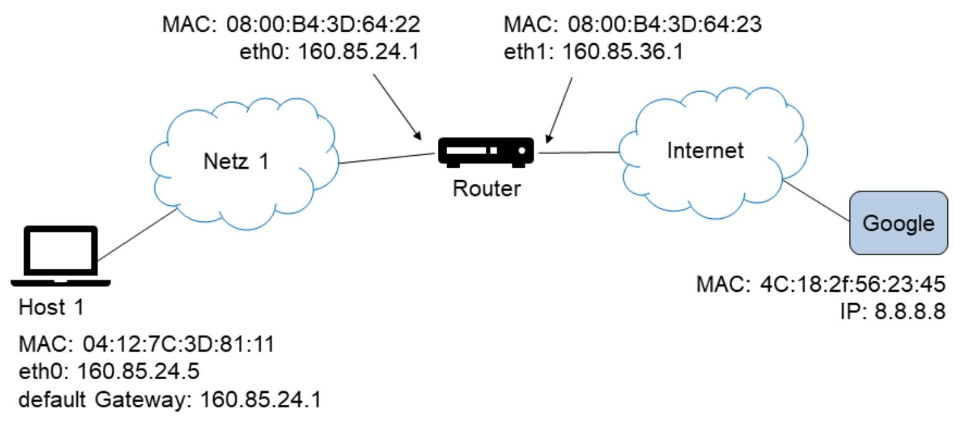
\includegraphics[width=0.9\linewidth]{images/images/arp_bsp.png}
  
  Geben Sie in der Tabelle jeweils die letzte HEX-Zahl der MAC-adresse oder die letzten zwei Dezimalzahlen der IP-Adresse an.

  \vspace{1mm}

  \resizebox{\linewidth}{!}{
\begin{tabular}{|l|l|l|l|l|l|}
\hline Request Typ & MACsrc & MACdest & IPsrc & IPdest & What \\
\hline ARP Request & 11 & FF & - & - & Who has IP 24.1 \\
\hline ARP Reply & 22 & 11 & - & - & 24.1 has 22 \\
\hline IP Paket & 11 & 22 & 24.5 & 8.8.8.8 & - \\
\hline
\end{tabular}}
\end{example2}

\subsection*{Transport Layer}

\begin{example2}{TCP Zustandsdiagramm}

  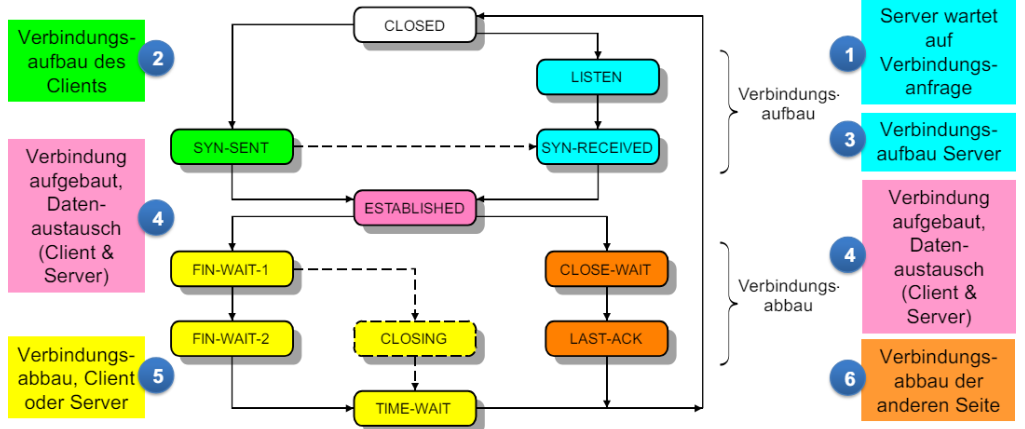
\includegraphics[width=1\linewidth]{images/images/zustandsdiagramm_tcp.png}
\end{example2}

\begin{example2}{TCP Sliding Window}
Zwei Hosts sind mit einem Duplex-Übertragungskanal von 1 GBit/s verbunden. Welche Übertragungsrate kann man mit einer TCP-Verbindung maximal erreichen, falls die Window Size auf 64 kByte begrenzt ist und die Round Trip Time $2 \mathrm{~ms}$ beträgt.

Der Overhead der Protokoll-Header kann bei dieser Betrachtung vernachlässigt werden. Unter welchen Bedingungen wird diese maximale Rate auch erreicht?

\begin{minipage}{0.4\linewidth}
  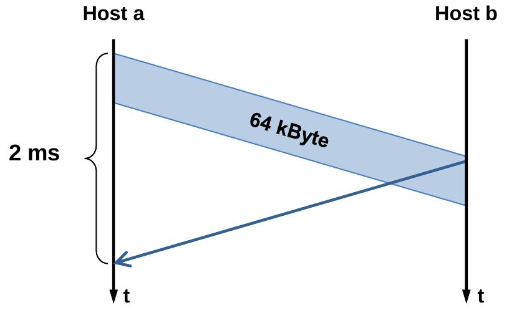
\includegraphics[width=1\linewidth]{images/images/tcp_slidingwindow.png}
\end{minipage}
\begin{minipage}{0.6\linewidth}
  \textbf{Antwort:}
Übertragungsrate $=64$ kByte alle $2 \mathrm{~ms}=64$ kByte * 8 Bit/Byte $/ 2 \mathrm{~ms}=256$ Mbit/s Damit ist der Kanal nur zu ca. $1 / 4$ der Zeit genutzt.
\end{minipage}

Diese theoretische Obergrenze wird nur dann erreicht, falls

- im Netz keine Paketverluste auftreten (würde als Congestion interpretiert und die Datenrate bremsen)

- Sender und Empfänger über genügend Leistung verfügen
  
\end{example2}

\subsection*{Application Layer}

\begin{example2}{NAT und Port Mapping}
Gegeben sei die Konfiguration gemäss untenstehendem Bild: Ein lokales IP-Netz 10.0.0.0/8 mit Host a und Host b, das über einen NAT Gateway und das Internet mit dem Host c verbunden sei:

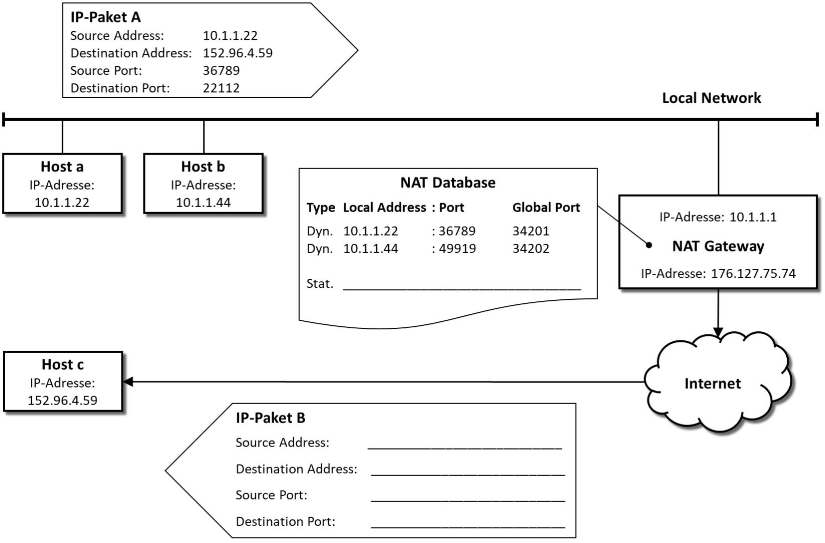
\includegraphics[width=1\linewidth]{images/images/nat_bsp.png}

Host a will das obige IP-Paket A an den Host c im Internet senden. Der NAT Gateway empfängt das IP-Paket A und schickt es als IP-Paket B an den Host c weiter.

a) Geben Sie oben die Source- und Destination-Adressen sowie die Source- und Destination-Ports des IP-Pakets B an.

\emph{IP Paket B:}

Source Address: 176.127 .75 .74

Destination Address: 152.96.4.59

Source Port: 34201

Destination Port: 22112

\vspace{1mm}

b) Der Host b soll dem Host c als TFTP Server dienen. Wie muss dazu der statische Eintrag in der NAT Database lauten? 

Hinweis: TFTP nutzt das UDP Port 69.

\vspace{1mm}

\begin{tabular}{lll} 
Type & Local Address: Port & Global Port \\
Static & 10.1.1.44:69 & 69
\end{tabular}
\end{example2}
